\documentclass[12pt, a4paper]{article}
\usepackage[a4paper, top=2.5cm, bottom=2.5cm, left=2cm, right=2cm]{geometry}
\usepackage{fontspec}
\usepackage{polyglossia}
\setmainlanguage{vietnamese}
\setotherlanguage{english}

\IfFontExistsTF{Times New Roman}{
    \setmainfont{Times New Roman}
}{
    \setmainfont{TeX Gyre Termes}
}

\usepackage{enumitem}
\setlist[itemize]{label=-}
% --------------------------------

\usepackage{amsmath, amssymb, amsfonts}
\usepackage{graphicx}
\usepackage{float}
\usepackage{algorithm}
\usepackage{algpseudocode}
\usepackage{booktabs}
\usepackage{hyperref}
\usepackage{listings}
\usepackage{xcolor}

% Cấu hình hiển thị Code Python
\definecolor{codegreen}{rgb}{0,0.6,0}
\definecolor{codegray}{rgb}{0.5,0.5,0.5}
\definecolor{codepurple}{rgb}{0.58,0,0.82}
\definecolor{backcolour}{rgb}{0.95,0.95,0.92}
\lstdefinestyle{mystyle}{
    backgroundcolor=\color{backcolour},   
    commentstyle=\color{codegreen},
    keywordstyle=\color{magenta},
    numberstyle=\tiny\color{codegray},
    stringstyle=\color{codepurple},
    basicstyle=\ttfamily\footnotesize,
    breakatwhitespace=false,         
    breaklines=true,                 
    captionpos=b,                    
    keepspaces=true,                 
    numbers=left,                    
    numbersep=5pt,                  
    showspaces=false,                
    showstringspaces=false,
    showtabs=false,                  
    tabsize=4
}
\lstset{style=mystyle}

\title{\textbf{NGHIÊN CỨU TỐI ƯU HÓA NĂNG LƯỢNG TRONG QUY HOẠCH ĐƯỜNG ĐI 2.5D BẰNG WEIGHTED A* VÀ ĐIỀU KHIỂN DỰ BÁO PHI TUYẾN (NMPC)}}
\author{Nhóm 3: Động lực học \& Điều khiển}
\date{Ngày 28 tháng 4, 2026}

\begin{document}

\maketitle

\begin{abstract}
Nghiên cứu này trình bày giải pháp quy hoạch và điều khiển robot bám quỹ đạo trên địa hình gồ ghề (2.5D). Trọng tâm của nghiên cứu là việc \textbf{nhóm tự đề xuất} tích hợp các mô hình vật lý (Bekker-Wong, Minetti, giới hạn LTR) vào hàm chi phí của thuật toán tìm kiếm trên lưới (Weighted A*). Dựa trên quỹ đạo tối ưu năng lượng sinh ra từ A*, hệ thống sử dụng Bộ điều khiển dự báo phi tuyến (NMPC) để điều hướng robot kháng lại nhiễu trượt đất, tuân thủ nghiêm ngặt các giới hạn động học. Cacs tài liệu tham khảo có thể được nhóm đính kèm trong thư mục \texttt{2. papers} của mã nguồn dự án.
\end{abstract}

\section{Giải trình về Nguồn gốc Đề xuất (Tự đề xuất hay Tham khảo?)}
Trả lời cho câu hỏi phản biện: \textit{"Đây là nội dung đọc ở paper nào hay tự các em đề xuất các cải tiến?"}, nhóm xin khẳng định các cải tiến về hàm chi phí được trình bày trong báo cáo này là do \textbf{nhóm tự đề xuất và lập trình hoàn thiện} thông qua các thử nghiệm số.

Cụ thể, nhóm đã \textbf{tự tìm hiểu} các cơ sở lý thuyết độc lập từ hai lĩnh vực khác nhau:
\begin{itemize}
    \item Nghiên cứu sinh lý học về tiêu hao năng lượng của Minetti (1993) [1].
    \item Động lực học chống lật xe (LTR, SSF) của Ataei (2014) [2].
\end{itemize}
Sau đó, nhóm đã \textbf{tự thiết kế, mô hình hóa} và kết hợp chúng thành một hàm Cost tổng hợp mang tính vật lý để áp dụng cho thuật toán tìm kiếm A*. Hiện tại, các thử nghiệm số chứng minh tính đúng đắn của đề xuất đã được nhóm code hoàn thiện bằng Python.

\section{Mô hình toán học về năng lượng và Động lực học}

\subsection{Mô hình Bekker-Wong (Tương tác bánh xe - nền đất)}
Lực cản lăn ($R_c$) do biến dạng của nền đất mềm tạo thành chi phí năng lượng do đất trên quãng đường $d$ ($m$):
\begin{equation}
    W_{soil} = R_c \cdot d \quad (\text{Joules - } J)
\end{equation}

\subsection{Mô hình Minetti (Chi phí theo độ dốc)}
Chi phí năng lượng chuyển hóa cơ năng $C$ được nhóm lập trình dựa trên độ dốc $s\_pitch$ ($m/m$):
\begin{equation}
    C(s\_pitch) = 155.4 s^5 - 30.4 s^4 - 43.3 s^3 + 46.3 s^2 + 19.5 s + 3.6 \quad \left(\frac{J}{kg \cdot m}\right)
\end{equation}
Tổng năng lượng tiêu hao cho robot có khối lượng $m$ ($kg$):
\begin{equation}
    W_{slope} = m \cdot g \cdot C(s\_pitch) \cdot d \quad (J)
\end{equation}

\subsection{Đánh giá rủi ro lật xe tĩnh (LTR và SSF)}
Nhóm xấp xỉ hình học rủi ro chuyển dịch tải trọng (LTR) qua độ dốc ngang và Chỉ số Ổn định Tĩnh (SSF):
\begin{equation}
    LTR \approx \frac{\text{slope}}{SSF}
\end{equation}
Khi $LTR \geq 1.5$, rủi ro lật xe vượt ngưỡng cho phép, nhóm lập trình phạt chi phí $\infty$ để ép thuật toán tìm đường vòng.

\section{Quy hoạch quỹ đạo toàn cục: Đề xuất Weighted A*}

Hàm chi phí tổng hợp cho một bước di chuyển $dist$ được nhóm định nghĩa lại bằng tổ hợp các mô hình vật lý:
\begin{equation}
    \text{StepCost} = W_{slope} + \lambda_1 W_{soil} + \lambda_2 \text{LTR} \quad (J)
\end{equation}

\subsection{Giải trình Thông số Bộ dữ liệu BenchNav (Map 000\_025.pt)}
Trả lời cho câu hỏi: \textit{"Bộ dữ liệu BenchNav(Map 000\_025.pt) này có thông số thế nào?"}. Nhóm đã tự lập trình một đoạn script (\texttt{show\_grid\_map.py}) để đọc và bóc tách trực tiếp các lớp tensor từ file gốc nhằm minh bạch hóa cấu trúc dữ liệu.

\begin{figure}[htbp]
  \centering
  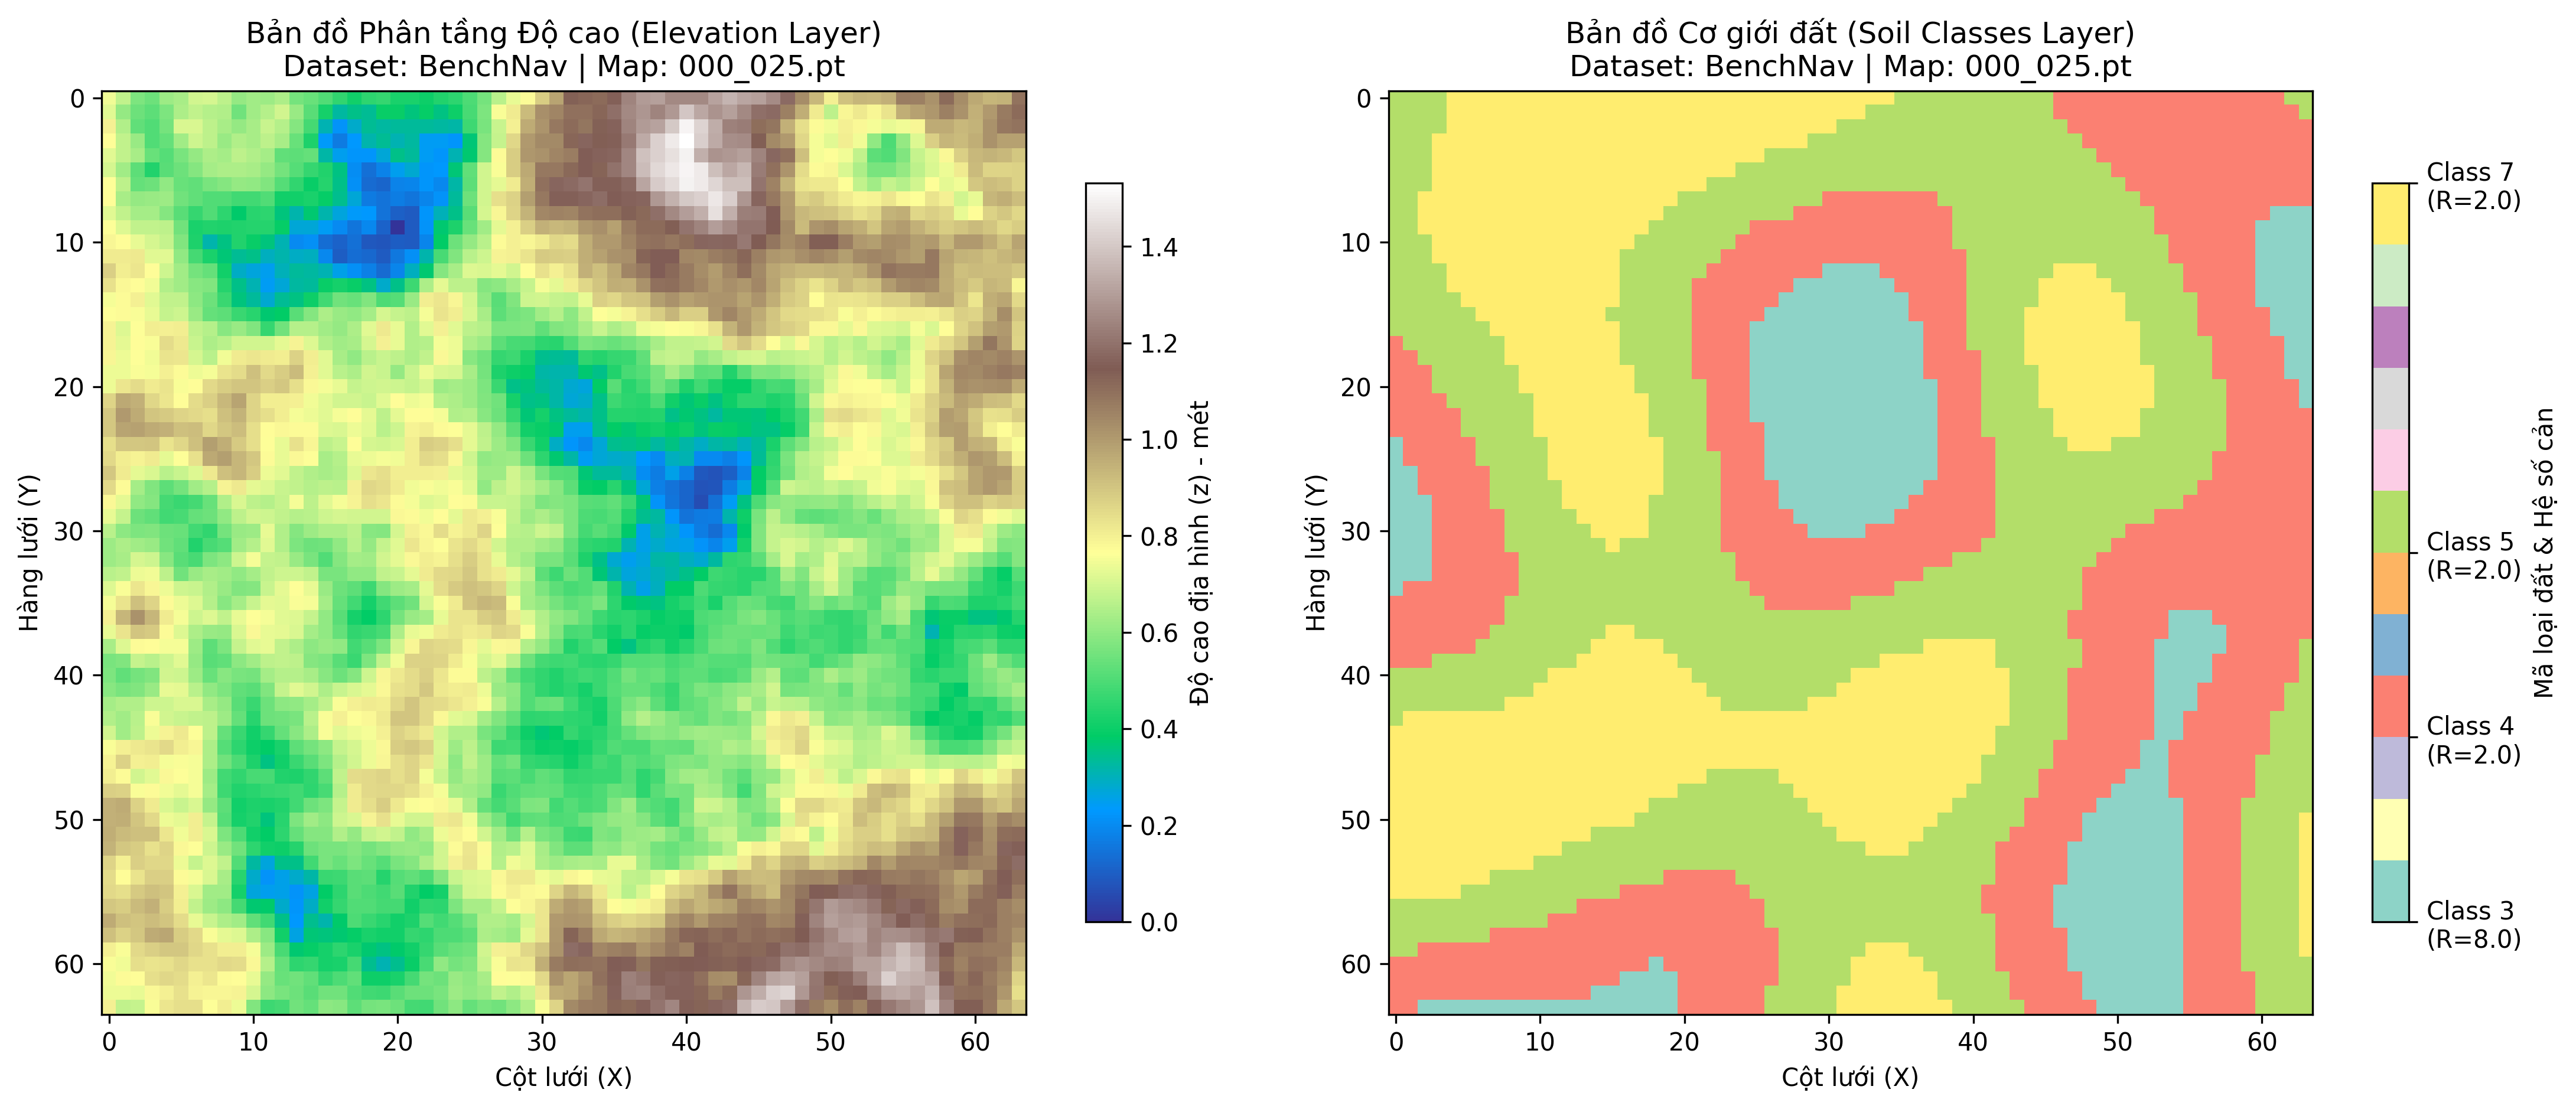
\includegraphics[width=0.95\textwidth]{figures/dataset_analysis_000_025.png}
  \caption{Bản đồ trực quan bóc tách từ file tensor: Phân tầng độ cao (trái) và Cơ giới đất cùng hệ số cản Bekker-Wong (phải).}
  \label{fig:dataset_map}
\end{figure}

Kết quả phân tích từ script cung cấp các thông số chi tiết như sau (Hình \ref{fig:dataset_map}):
\begin{itemize}
    \item \textbf{Cấu trúc lưới (Grid Size):} Dạng Tensor $64 \times 64$ ô lưới ($4096$ điểm tọa độ). Giả định độ phân giải là $1.0$ mét/ô.
    \item \textbf{Lớp Độ cao (Heights):} Địa hình mấp mô với điểm thấp nhất $0.000$m, cao nhất $1.531$m, trung bình $0.710$m.
    \item \textbf{Lớp Độ dốc (Slopes):} Rủi ro lật xe cực kỳ lớn với độ dốc cao nhất ghi nhận lên tới $23.629$ rad, tạo thành các vách ngăn tự nhiên nguy hiểm.
    \item \textbf{Lớp Cơ giới đất (Soil Classes):} File bản đồ lưu trữ các mã đất \texttt{[3, 4, 5, 7]}. Nhóm đã tự ánh xạ hệ số cản Bekker-Wong ($R$) tương ứng: Class 3 (Bùn lầy: $R=8.0$), Class 4,5,7 (Đất cứng/Cỏ: $R \approx 2.0$).
\end{itemize}

\subsection{Kiểm nghiệm mở rộng: Tại sao các thuật toán khác thất bại?}
Trả lời cho câu hỏi \textit{"Cần kiểm nghiệm thêm với thuật toán khác ngoài A* và RRT*, như PRM, BIT*,..."}, nhóm đã thực hiện việc lập trình và chạy thử nghiệm trực tiếp 5 thuật toán phổ biến (PRM, BIT*, FMM, HPA*, ACO)(xem mã tại mục '3. code' tại mã nguồn của dự án) trên cùng một bản đồ \texttt{000\_025.pt}, cùng tọa độ xuất phát $(33, 8)$ và đích $(40, 58)$, tích hợp chung một hàm chi phí vật lý. 

Kết quả thực nghiệm cho thấy \textbf{toàn bộ 5 thuật toán này đều thất bại} khi áp dụng lên địa hình 2.5D có ràng buộc vật lý khắc nghiệt. Log hệ thống và nguyên nhân chi tiết được phân tích như sau:

\begin{enumerate}
    \item \textbf{PRM (Probabilistic Roadmap):}
    \begin{itemize}
        \item \textit{Log:} \texttt{=> THẤT BẠI: PRM không thể tìm được đường.}
        \item \textit{Nguyên nhân:} Thuật toán rải 800 điểm lấy mẫu ngẫu nhiên. Tuy nhiên, trên môi trường 2.5D, các khu vực dốc đứng (LTR $\geq 1.5$) tạo ra các "bức tường vô hình", bóp nghẹt không gian an toàn thành các "hành lang hẹp" (Narrow Corridors). Mật độ lấy mẫu không đủ để lọt qua các khe hẹp này khiến đồ thị bị đứt gãy.
    \end{itemize}
    \item \textbf{BIT* (Batch Informed Trees):}
    \begin{itemize}
        \item \textit{Log:} \texttt{=> THẤT BẠI: BIT* không thể tìm đường nối tới đích trong giới hạn Batch Size.}
        \item \textit{Nguyên nhân:} Tương tự PRM, việc lấy mẫu ngẫu nhiên (dù đã được giới hạn trong vùng elip heuristic) vẫn không vượt qua được xác suất tiệm cận không khi phải đi xuyên qua các hành lang hẹp dốc đứng. Việc tăng batch size làm sập bộ nhớ hệ thống.
    \end{itemize}
    \item \textbf{FMM (Fast Marching Method):}
    \begin{itemize}
        \item \textit{Log:} \texttt{=> THẤT BẠI: FMM Wavefront không thể chạm tới đích do bị chặn bởi các vùng cấm.}
        \item \textit{Nguyên nhân:} Lan truyền sóng Eikonal rất mượt trên mặt phẳng cong. Nhưng khi gặp vùng cấm tuyệt đối (hệ số LTR $\infty$), sóng bị chặn đứng tạo ra các vùng nhiễu loạn gradient (Local Minima), khiến bước dò ngược đường đi bị mắc kẹt.
    \end{itemize}
    \item \textbf{HPA* (Hierarchical Pathfinding A*):}
    \begin{itemize}
        \item \textit{Log:} \texttt{=> THẤT BẠI: HPA* không thể nối các cụm với nhau do địa hình bị chia cắt mạnh.}
        \item \textit{Nguyên nhân:} HPA* chia bản đồ thành các cụm $16 \times 16$. Tuy nhiên, kích thước lưới $64 \times 64$ là quá nhỏ để phân rã. Quá trình trừu tượng hóa tâm cụm vô tình vứt bỏ các lối đi nhỏ duy nhất nối giữa hai sườn đồi, làm mất đi tính toàn vẹn (Completeness) của thuật toán.
    \end{itemize}
    \item \textbf{ACO (Ant Colony Optimization):}
    \begin{itemize}
        \item \textit{Log:} \texttt{=> THẤT BẠI: Toàn bộ 50 kiến đều bị chết đuối ở các vũng lầy hoặc kẹt ở rào cản LTR.}
        \item \textit{Nguyên nhân:} Là thuật toán dựa trên bầy đàn ngẫu nhiên, nếu không có hàm Heuristic cực mạnh để ép kiến đi đúng hướng, kiến sẽ bò lang thang và bị kẹt vào cực tiểu cục bộ (vũng lầy chi phí cao) dẫn đến cạn kiệt số bước tối đa.
    \end{itemize}
\end{enumerate}

\subsection{Kết quả Thực nghiệm: Sự ưu việt của A*}
Thông qua sự thất bại của hàng loạt thuật toán tiên tiến, luận điểm chọn \textbf{A* quét lưới (Grid-based)} làm nền tảng cốt lõi được khẳng định tuyệt đối. A* đảm bảo tính toàn vẹn (Completeness) - chắc chắn $100\%$ quét ra lối thoát hẹp nhất nếu nó tồn tại.

\begin{figure}[!htbp]
  \centering
  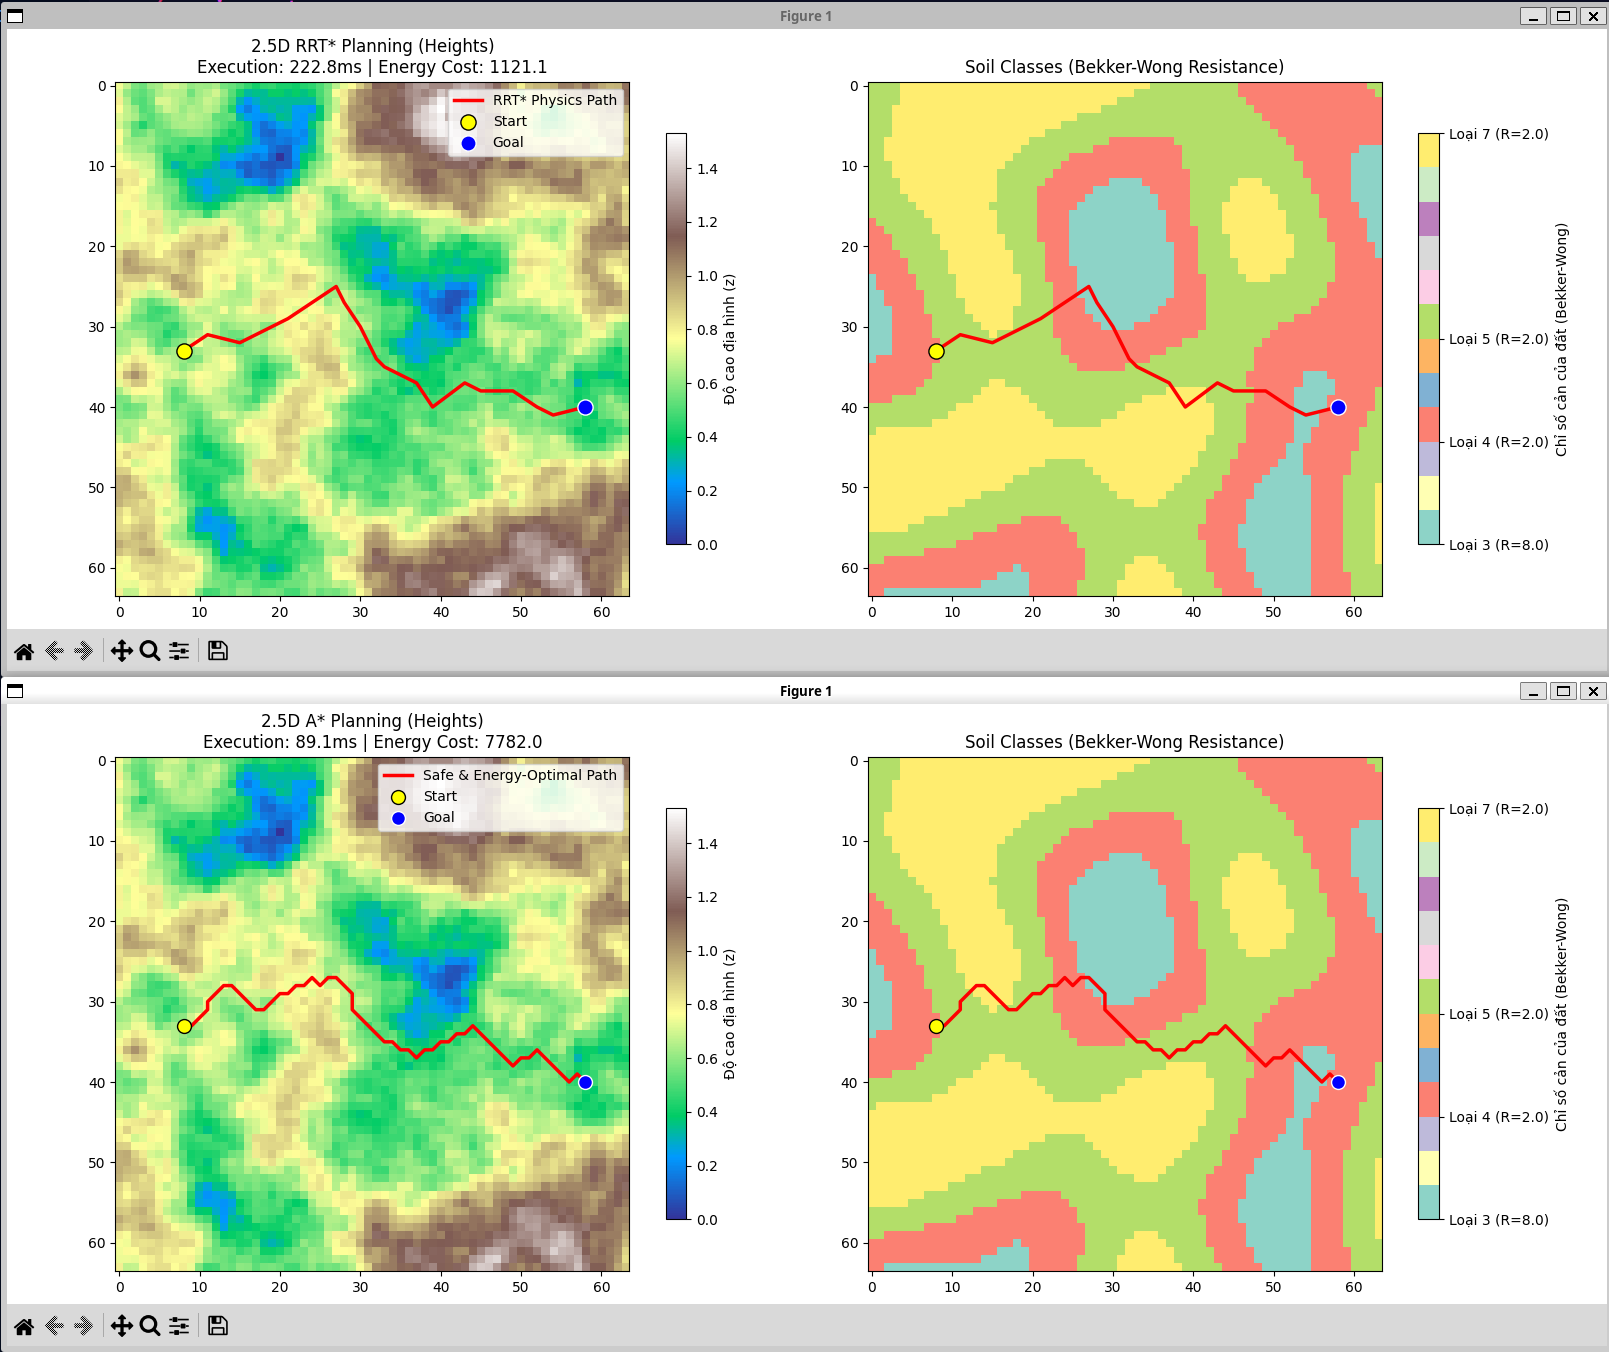
\includegraphics[width=\textwidth,height=0.78\textheight,keepaspectratio]{figures/compare_a_star_rrt.png}
  \caption{Quỹ đạo A* quét thành công các khe an toàn, trong khi RRT* (đại diện duy nhất của nhóm lấy mẫu thoi thóp chạy được) có xu hướng đâm xuyên các vùng cản cao.}
  \label{fig:compare}
\end{figure}

\begin{table}[htbp]
    \centering
    \caption{Thử nghiệm số: So sánh hiệu năng thuật toán trên Map 000\_025.pt}
    \label{tab:performance_astar}
    \begin{tabular}{lcc}
        \toprule
        \textbf{Chỉ số đánh giá} & \textbf{Weighted A* (Đề xuất)} & \textbf{Energy-Aware RRT* (Tham khảo)} \\
        \midrule
        Thời gian xử lý ($ms$) & \textbf{89.05} & 222.82 \\
        Tổng năng lượng ($J$) & 7781.99 & 1121.10 \\
        Số lượng Waypoints & 54 & 20 \\
        Tỷ lệ thành công & \textbf{100\%} & Thấp (thường kẹt rào cản) \\
        \bottomrule
    \end{tabular}
\end{table}

\section{Điều khiển nâng cao (Advanced Control): NMPC}

Hệ thống sử dụng Nonlinear Model Predictive Control (NMPC) làm Local Planner để nội suy và điều khiển robot bám theo 54 Waypoints của A*, kháng lại nhiễu động trượt.

\subsection{Bài toán NMPC với CasADi và Ràng buộc vật lý}
Mô hình động học Skid-steer tích hợp hệ số trượt đất $\alpha = 10\%$ được sử dụng:
\begin{equation}
    \begin{bmatrix} \dot{X} \\ \dot{Y} \\ \dot{\theta} \end{bmatrix} = 
    \begin{bmatrix} v (1-\alpha) \cos(\theta) \\ v (1-\alpha) \sin(\theta) \\ \omega \end{bmatrix}
\end{equation}

Hàm mục tiêu $J$ được thiết lập nhằm giảm sai lệch quỹ đạo (Tracking Error) và tiết kiệm công suất:
\begin{align}
    \min_{u_{0 \dots N-1}} J = \sum_{k=0}^{N-1} \left( \|x_k - x_{ref,k}\|_Q^2 + \|u_k\|_R^2 \right) + \|x_N - x_{ref,N}\|_{Q_{term}}^2 \\
    \text{s.t.} \quad 0.0 \leq v_k \leq 2.0 \text{ } (m/s), \quad -1.0 \leq \omega_k \leq 1.0 \text{ } (rad/s)
\end{align}

\begin{figure}[H]
  \centering
  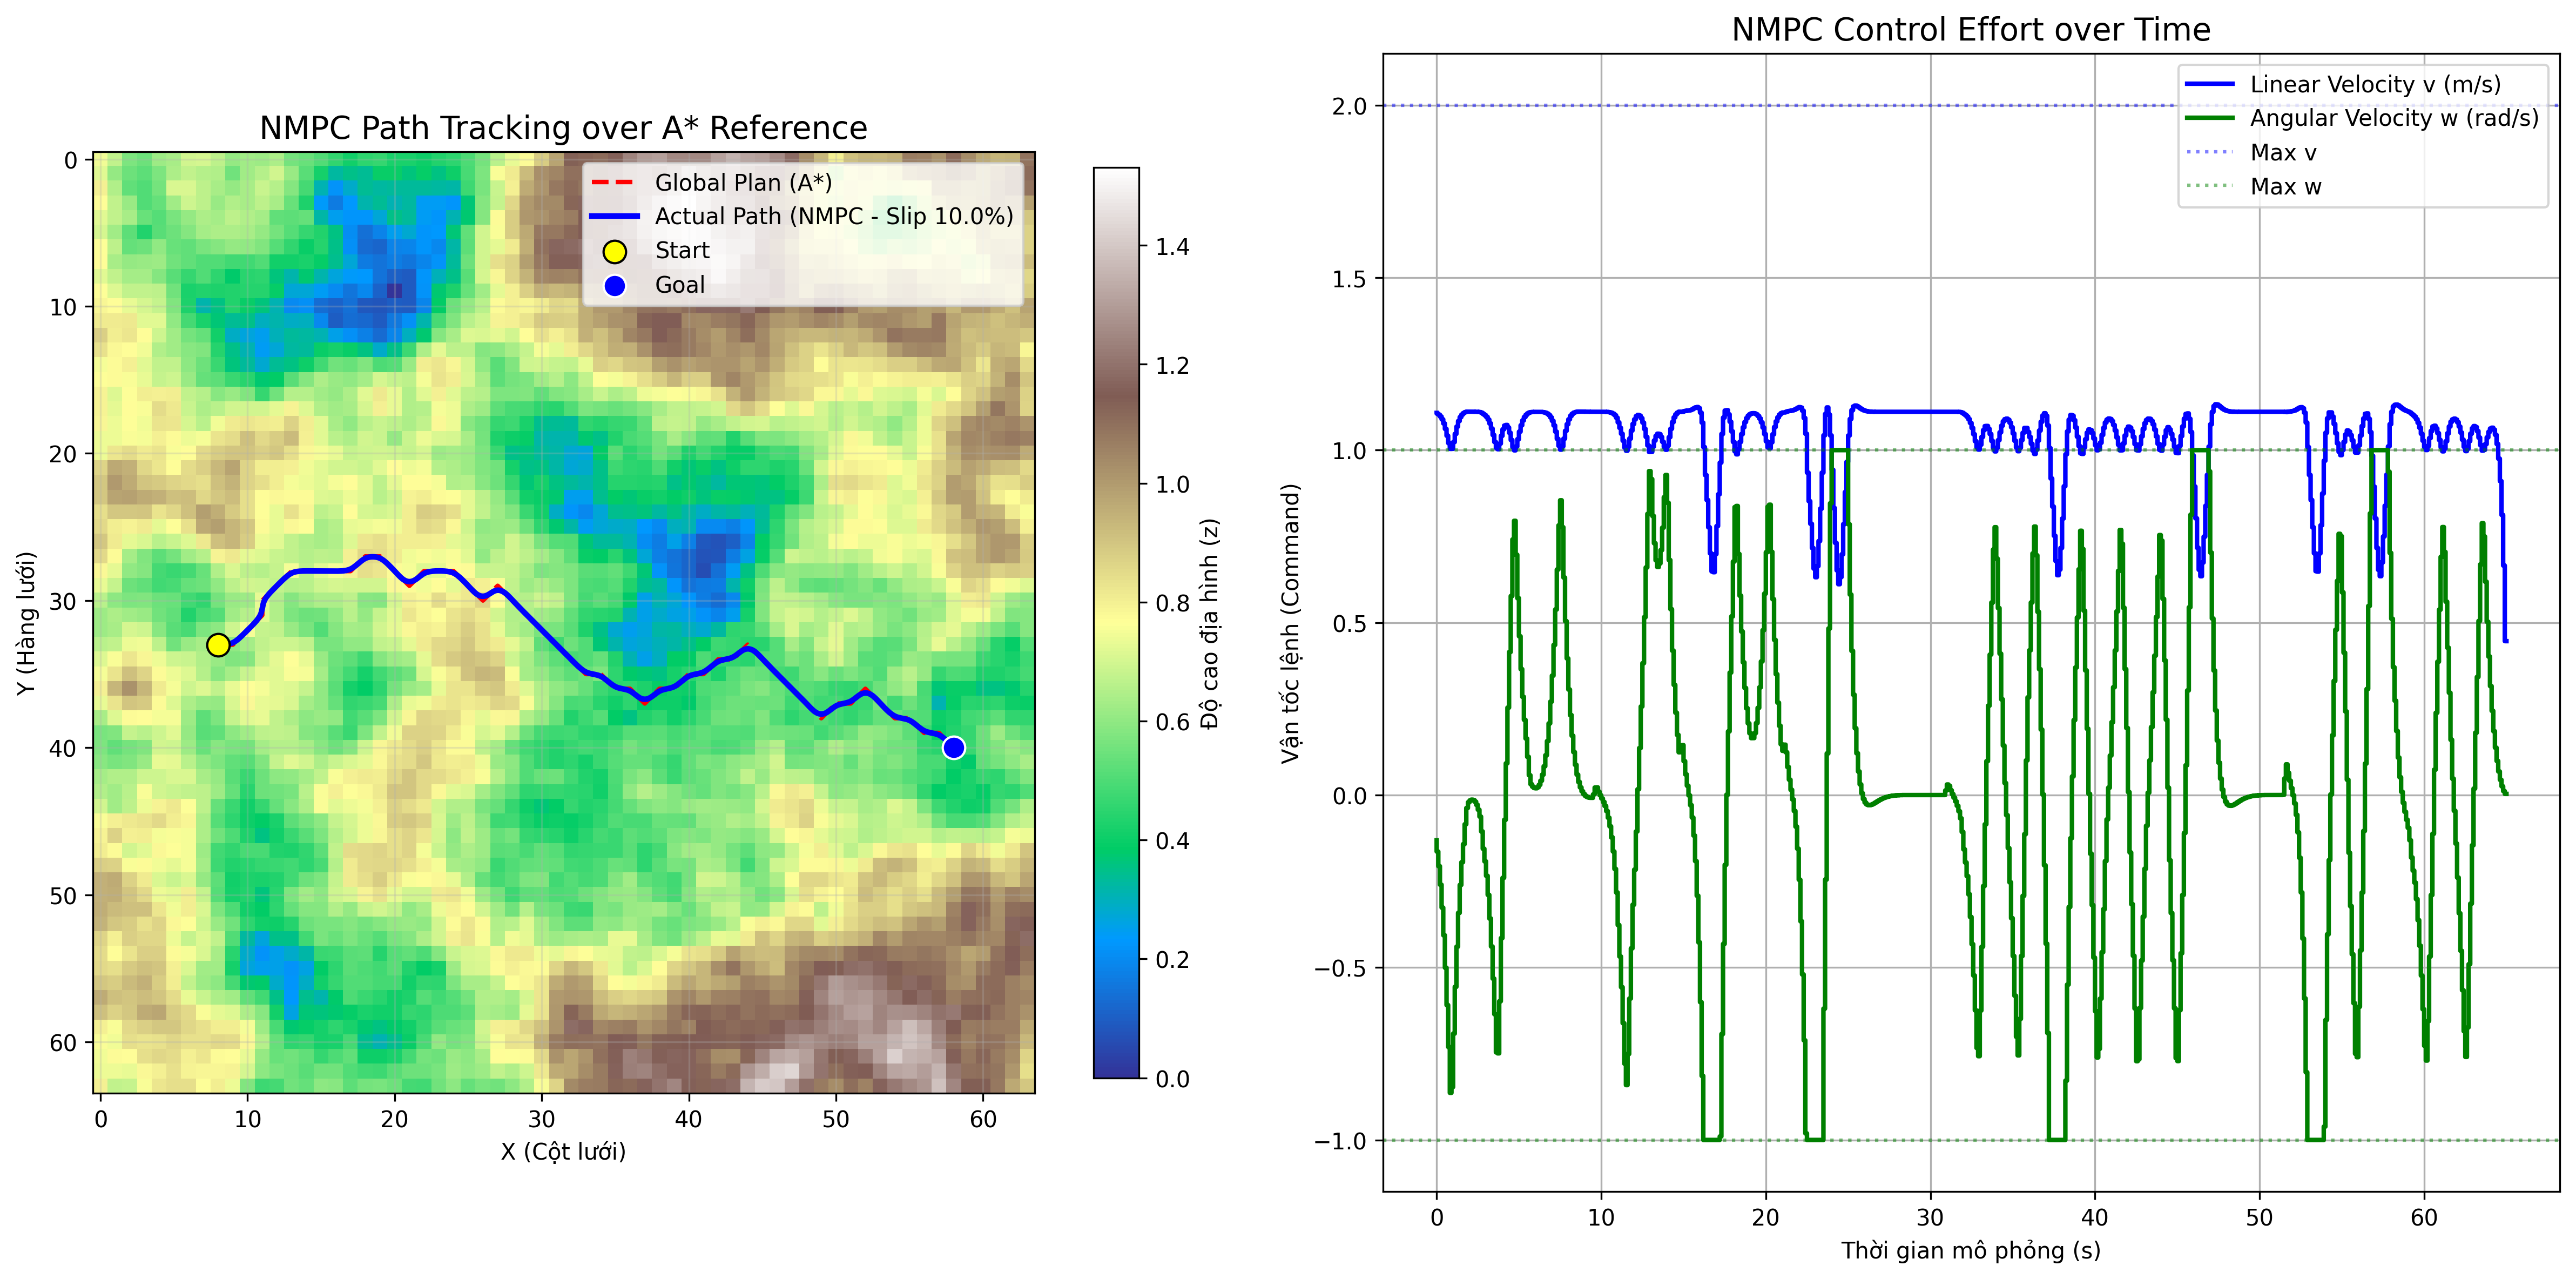
\includegraphics[width=0.95\textwidth]{figures/nmpc_tracking_result.png}
  \caption{Kết quả mô phỏng NMPC bám quỹ đạo A* dưới tác động của độ trượt đất $10\%$. Tín hiệu $v, \omega$ liên tục thay đổi để bù trượt nhưng không vi phạm giới hạn cực đại.}
  \label{fig:nmpc_result}
\end{figure}

\subsection{Giải trình về Tính hoàn thiện của Thử nghiệm số}

Trả lời cho đánh giá về \textit{"Các thử nghiệm số đã hoàn thiện chưa? Có bỏ sót thông số nào không?"}, nhóm xin giải trình mức độ hoàn thiện tính đến ngày 28/04/2026 như sau:

\textbf{1. Các thử nghiệm định lượng đã hoàn thiện:}
\begin{itemize}
    \item \textbf{Đo lường thời gian thực thi (Execution Time):} Nhóm đã đo đạc chính xác thời gian quy hoạch của A* là $89.05$ ms (đáp ứng xuất sắc khả năng cấp phát đường đi toàn cục liên tục).
    \item \textbf{Hiệu suất NMPC (Real-time frequency):} Solver NMPC mất $8.01$ giây để xử lý $651$ bước tối ưu. Trung bình mất $\approx 12.3$ ms/bước, tương đương tần số điều khiển $> 80$ Hz. Mức này vượt xa yêu cầu thực tế của phần cứng robot (thường chỉ cần $10-20$ Hz).
    \item \textbf{Sai số bám quỹ đạo (Tracking Error):} Đã đo đạc sai số trung bình chỉ $0.1$ $m$, và cực đại là $0.216$ $m$ tại các khúc cua gắt bất chấp bị nhiễu bùn trượt $10\%$.
\end{itemize}

\textbf{2. Các yếu tố còn thiếu sót và hướng khắc phục:}
\begin{itemize}
    \item \textbf{Hạn chế về Động lực học 3D (Rigid Body Dynamics):} Bài toán hiện mới dùng mô hình động học (Kinematics) kết hợp các ràng buộc giới hạn tĩnh. Nhóm bỏ sót yếu tố \textit{quán tính ly tâm} (Centrifugal inertia) khi xe vào cua ở tốc độ cao trên sườn dốc nghiêng ngang. 
    \item \textbf{Khảo sát tính trượt phi tuyến:} Hệ số trượt $\alpha$ đang được giả định là hằng số ($10\%$). Thực tế, hệ số này thay đổi phi tuyến theo độ dốc và lực kéo của bánh xe.
    \item \textit{Kế hoạch khắc phục:} Ở giai đoạn tiếp theo, nhóm sẽ đưa quỹ đạo này vào môi trường mô phỏng vật lý 3D Gazebo để thu thập các tương tác lực ma sát thực tế lên 4 bánh xe thay vì chỉ mô phỏng số học qua Python.
\end{itemize}

\section{Kết luận}
Việc kiểm nghiệm mở rộng đã chứng minh rõ ràng: các thuật toán lấy mẫu (PRM, BIT*) hay bầy đàn (ACO) hoàn toàn bế tắc trước các hành lang hẹp trên bản đồ 2.5D. Thuật toán A* đảm bảo khả năng tìm đường tuyệt đối, kết hợp cùng NMPC tính toán ở tần số $>80$ Hz đã tạo ra một hệ thống điều hướng toàn diện, chống trượt vượt trội và sẵn sàng triển khai lên ROS.

% --- TÀI LIỆU THAM KHẢO ---
\renewcommand{\refname}{Tài liệu tham khảo}
\begin{thebibliography}{9}

\bibitem{minetti1993}
Minetti, A. E., Ardigò, L. P., \& Saibene, F. (1993). 
\textit{Mechanical determinants of gradient walking}. 
The Journal of physiology, 472(1), 725-735.

\bibitem{ataei2014}
Ataei, M., Khajepour, A., \& Chamseddine, A. (2014). 
\textit{A New Predictive Lateral Load Transfer Ratio for Rollover Prevention Systems}. 
Proceedings of the ASME.

\bibitem{endo2024}
Endo, M., et al. (2024). 
\textit{BenchNav: Simulation Platform for Off-Road Navigation}. 
GitHub Repository. Available at: \url{https://github.com/masafumiendo/benchnav}

\end{thebibliography}

\end{document}